\section{The Mathematical Contest in Modeling(MCM)}

So far, I have participated in the Mathematical Contest in Modeling three times, specifically in 2022 and 2023. In both competitions, I completed the writing of the competition papers and received \textbf{Honorable Mention awards}. The papers submitted for both competitions will be placed in an \textbf{attachment} for inspection.

In the Mathematical Contest in Modeling, the ability to learn new knowledge is an indispensable aspect. During the competition, paper writing and mathematical modeling abilities are improved, and most importantly, \textbf{the ability to learn new knowledge is enhanced}. Only by reading various types of papers can we better understand the background and requirements of the problem and optimize the model in a targeted manner. In addition, the competition also offers opportunities to practice previously learned skills, such as Python, Latex, Matlab, etc.

\subsection{Introduction to MCM 2022}
In the 2022 competition, we chose Problem A (Power Profile of a Cyclist). In this competition, my primary responsibilities included \textbf{model creation, partial model calculation, most paper writing, and subsequent Latex typesetting}.

Due to COVID-19 in 2022, we could not conduct offline mock competitions and could not return to school before the competition started. Under the constraint of limited time, I proposed a method to optimize the simple differential equation model through physical modeling and \textbf{established a differential equation predictive model based on force analysis}. Using data from online searches, we added a series of parameters to the differential equation model and carried out calculations, enabling the model to match existing cyclist data and various race tracks. Ultimately, we drew a \textbf{Power Profile and predicted the time} to complete the race. Upon testing, the prediction results of this model were consistent with the actual situation. Although this model's precision in predicting the intermediate process has some room for optimization, such as setting parameters as values rather than equations, it generally met the requirements of the problem and yielded satisfactory results.

\begin{figure}[H]
	\centering
	\includegraphics[width=0.7\linewidth]{"Introduction/figures/2022 MCM"}
	\caption{2022 Mathematical Contest in Modeling}
	\label{fig:2022-mcm}
\end{figure}

\subsection{Introduction to MCM 2023}
In the 2023 competition, we selected Problem B (Reimagining Maasai Mara). In this competition, my primary responsibilities included the first part of the question: \textbf{the Grid-Method, Logistic regression Model, and Economical models.} I also contributed to some \textbf{paper writing, Matlab plotting, and subsequent Latex typesetting}.

In this competition, we used the \textbf{Grid-Method} for regional planning. Reading related professional papers, we got the idea to define new parameters for regional division and separately establish models. Therefore, we defined the parameter "environmental sensitivity" to represent the impact of humans and the environment on animals and divided the region into three parts according to the impact from small to large. For different regions, we separately established \textbf{Logistic regression Models} and \textbf{Economical models} to predict population numbers and changes in natural resources. Subsequently, we used the Entropy weight method to formulate specific policies for each region. By collecting data on each region's population numbers and natural resources, we quantitatively analyzed the impacts to predict the equilibrium point of the harmonious coexistence of wildlife, nature, and humans. By verifying Maasai Mara data, we proved that our model fits well with the actual past situation and is suitable for prediction in this region. Finally, we \textbf{proposed specific policies} for different regions based on the analysis results and \textbf{made predictions}.

\begin{figure}[htp]
	\centering
	\includegraphics[width=0.7\linewidth]{"Introduction/figures/2023 MCM"}
	\caption{2023 Mathematical Contest in Modeling}
	\label{fig:2023-mcm}
\end{figure}

\section{Internship at the Guangdong Academy of Science}

From July to August 2022, \textbf{I interned at the Guangdong Academy of Science}. During my internship, my position was a Designer. Under my supervisor's and senior colleagues' guidance, I was responsible for designing and assembling parts of acoustic intelligent sensing devices using \textbf{SolidWorks}, and I also undertook some work with\textbf{ Visualize}.

During the internship, I gained new insights into mechanical engineering and related industries by learning about the latest industry trends and communicating with my colleagues. I believe that a contemporary mechanical engineer needs to possess three skills: \textbf{design and drawing, programming, and "bringing mechanics to life".}

The first is \textbf{mechanical design}: design and drawing are fundamental to the mechanical industry. The construction of all mechanical equipment relies on design and the verification of material performance. Only by creating each small mechanical component to meet design principles and usage requirements can it be assembled into a device that meets the standards. Next is \textbf{programming}. Nowadays, every industry relies on programs, and programming has become an indispensable auxiliary tool. For example, Python can not only simulate signals needed for sensor equipment using tools like Soundfile, but its data analysis tools, such as Numpy and Matplotlib, also have broad applicability. Finally, \textbf{"bringing mechanics to life"} means using specific tools to allow users to understand the usage and function of a device intuitively. A difficult-to-operate machine could potentially narrow its scope of application, while "bringing it to life" can prevent this situation and increase product recognition.

\begin{figure}
	\centering
	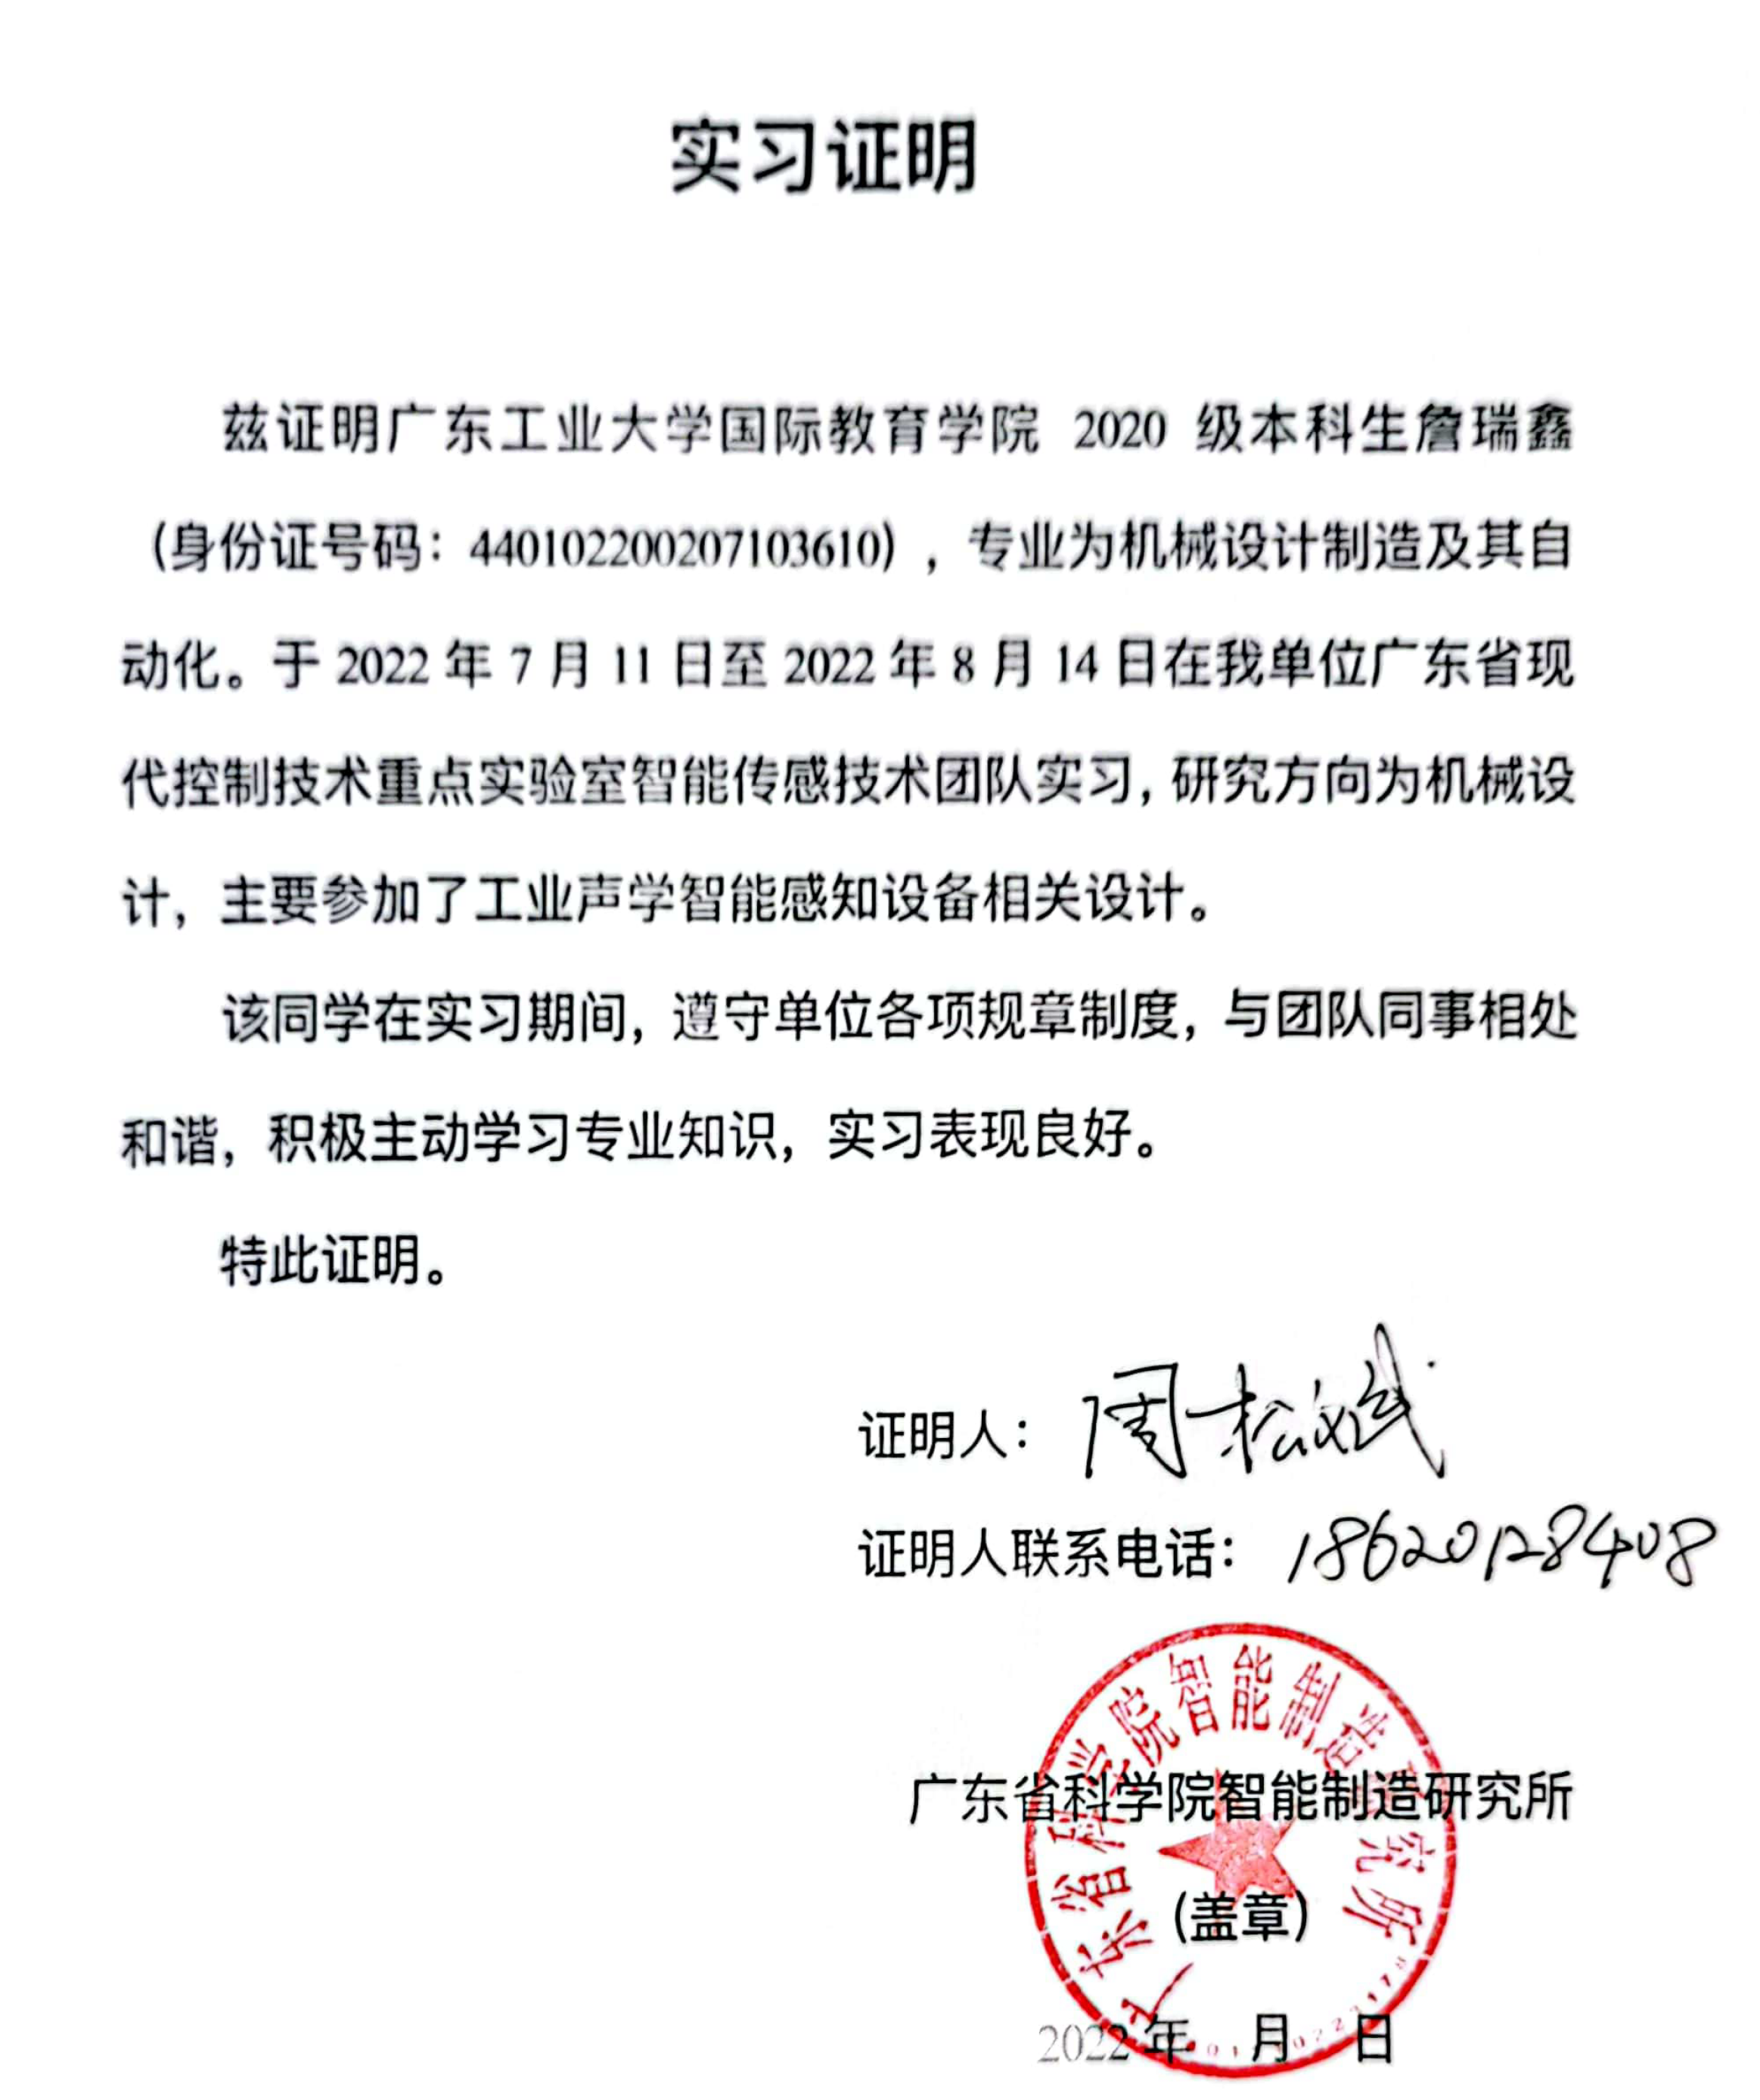
\includegraphics[width=0.5\linewidth]{Introduction/figures/实习}
	\caption{Internship Certificate}
	\label{fig:}
\end{figure}

\section{Work at the University of Exeter}

From November 2022 to the present, I have been employed by the University of Exeter as a \textbf{Digital Assistant and Student Ambassador}. During my employment, my primary responsibilities include \textbf{operating the university's social media accounts in China}, such as the official WeChat public account, Xiaohongshu, and Weibo, among others. Through social media channels, I promote the university, assist new students with their pre-enrollment steps, and answer inquiries from prospective and current students about the university. At the same time, I assist in various recruitment activities and shooting, collecting, and writing article materials. 

\begin{figure}[htp]
	\centering
	\subfloat{\includegraphics[width=8cm]{"Introduction/figures/3"}}
	\subfloat{\includegraphics[width=8cm]{"Introduction/figures/4"}}
	\\
	\centering
	\subfloat{\includegraphics[width=8cm]{"Introduction/figures/5"}}
	\subfloat{\includegraphics[width=8cm]{"Introduction/figures/6"}}
	\caption{Some media material shot} %图片标题
	\label{Fx}
\end{figure}

\label{sec:introduction}
\FloatBarrier % Now figures cannot float above section title